% Authors: DMason
\section{Signal Acceptance}
\label{sec:signalMC}

Here we look at signal acceptance for 5e32 (and later) triggers.

\subsection{GMSB global acceptance}

SUSY GMSB MC with a coarse grid in $m_{squark}$ = (600,800,1000,1500) GeV, $m_{gluino}$ = (700,900,1200,1600) GeV,
and $m_{wino}$ = (100,300,500) GeV.  The SLHA (ref) SUSY spectra files were generated with SUSPect (ref).
About 2500 events were generated at each grid point and run through the full detector simulation ("fullsim") 
using CMSSW\_3\_11\_1.  For this first study no photon enriching filtering was applied.

Figure \ref{fig:genphotons} shows what percentage of each of these 
generated bins included a generated "prompt" photon from the decay of a $\chi_0$.  One sees fluctuation
between the bins in $m_{squark}$ and $m_{gluino}$ due to statistics in the samples, and a general
trend towards a decreasing percentage of the sample containing prompt photons as the Wino mass increases.
With a Wino mass of 100 GeV the majority of the events include a photon resulting from $\chi_0$ decay.

 \begin{figure}[!ht]
  \centering
 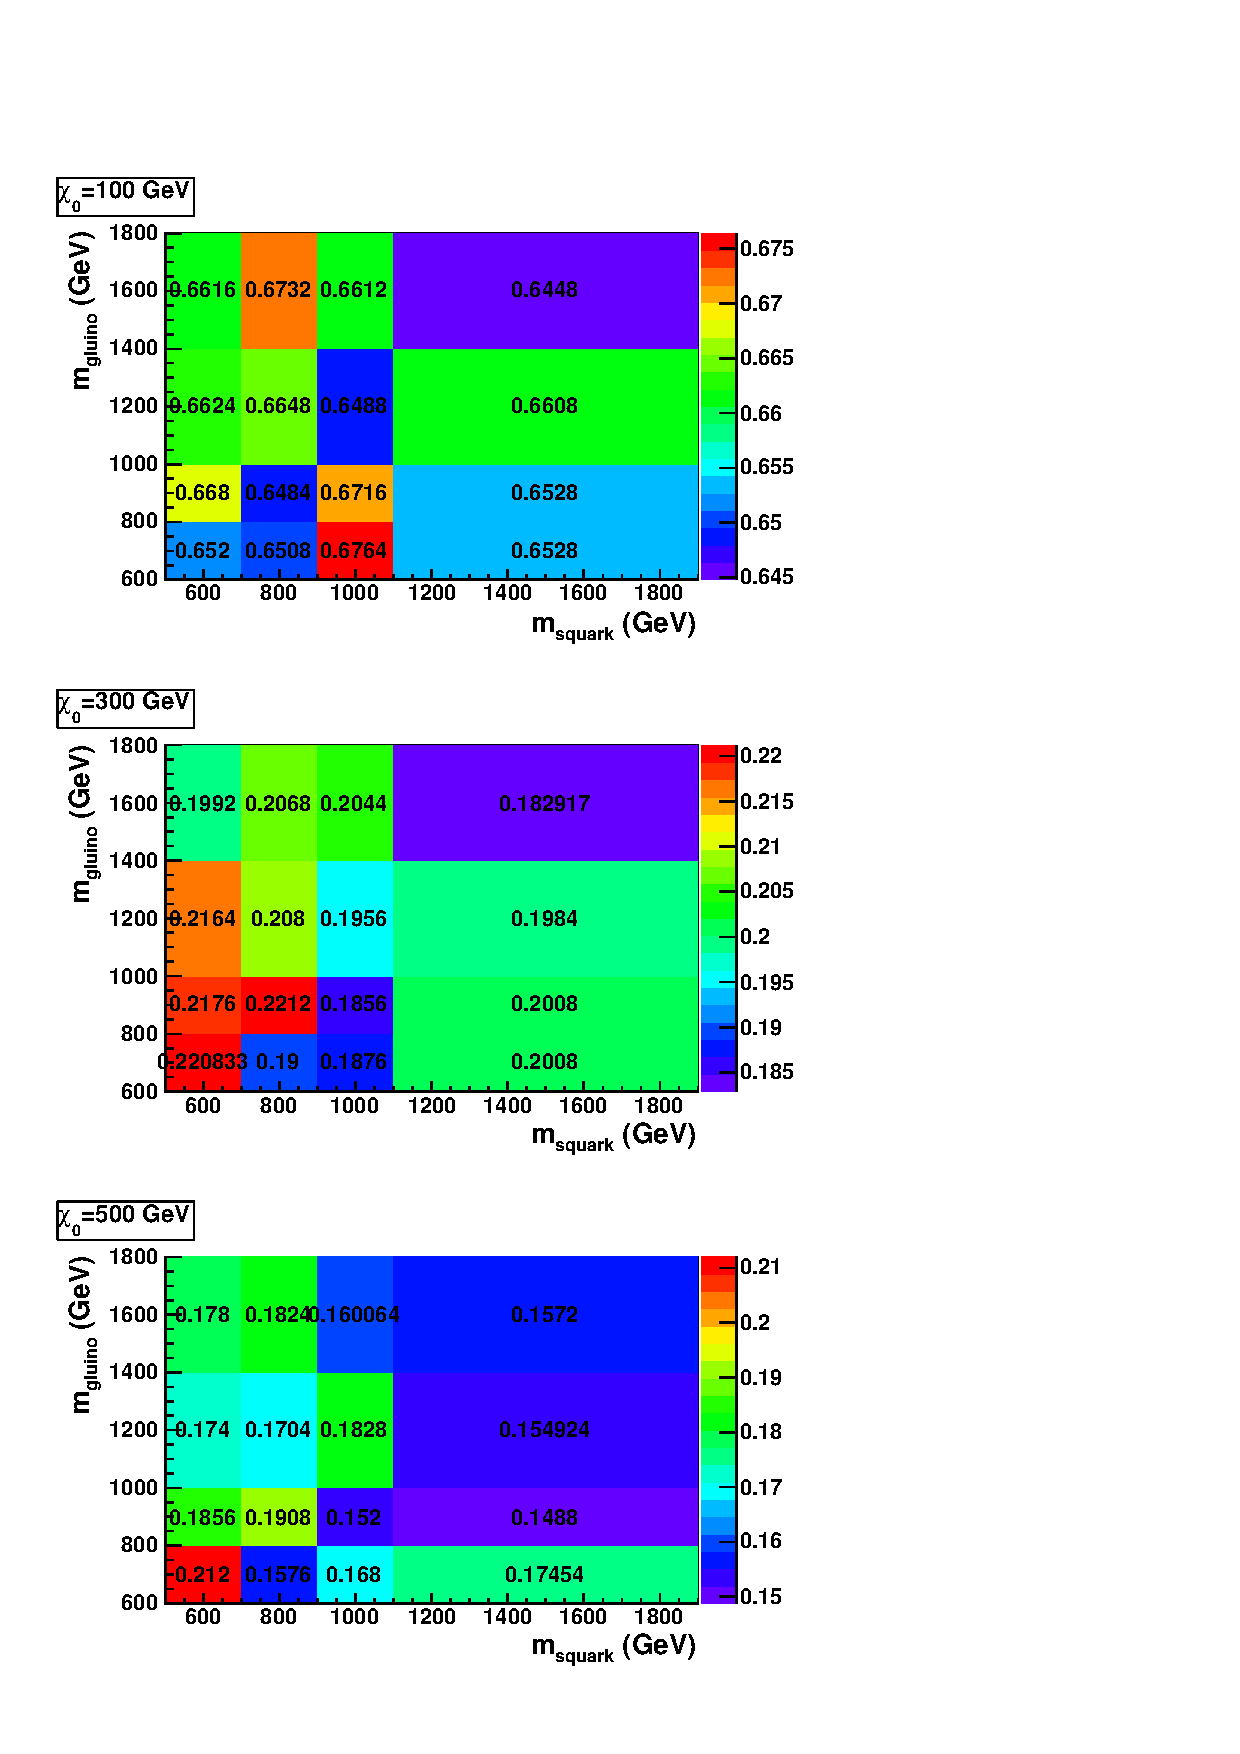
\includegraphics[width=0.5\textwidth]{figures/genphotonsnopu.pdf}
\caption{Percent of MC in each of the 48 bins which have a photon originating from a $\chi_0$.  The three
plots correspond to each of the three Wino mass bins.}
\label{fig:genphotons}
\end{figure}



\subsubsection{SUSY proposed triggers}

 \begin{figure}[!ht]
  \centering
 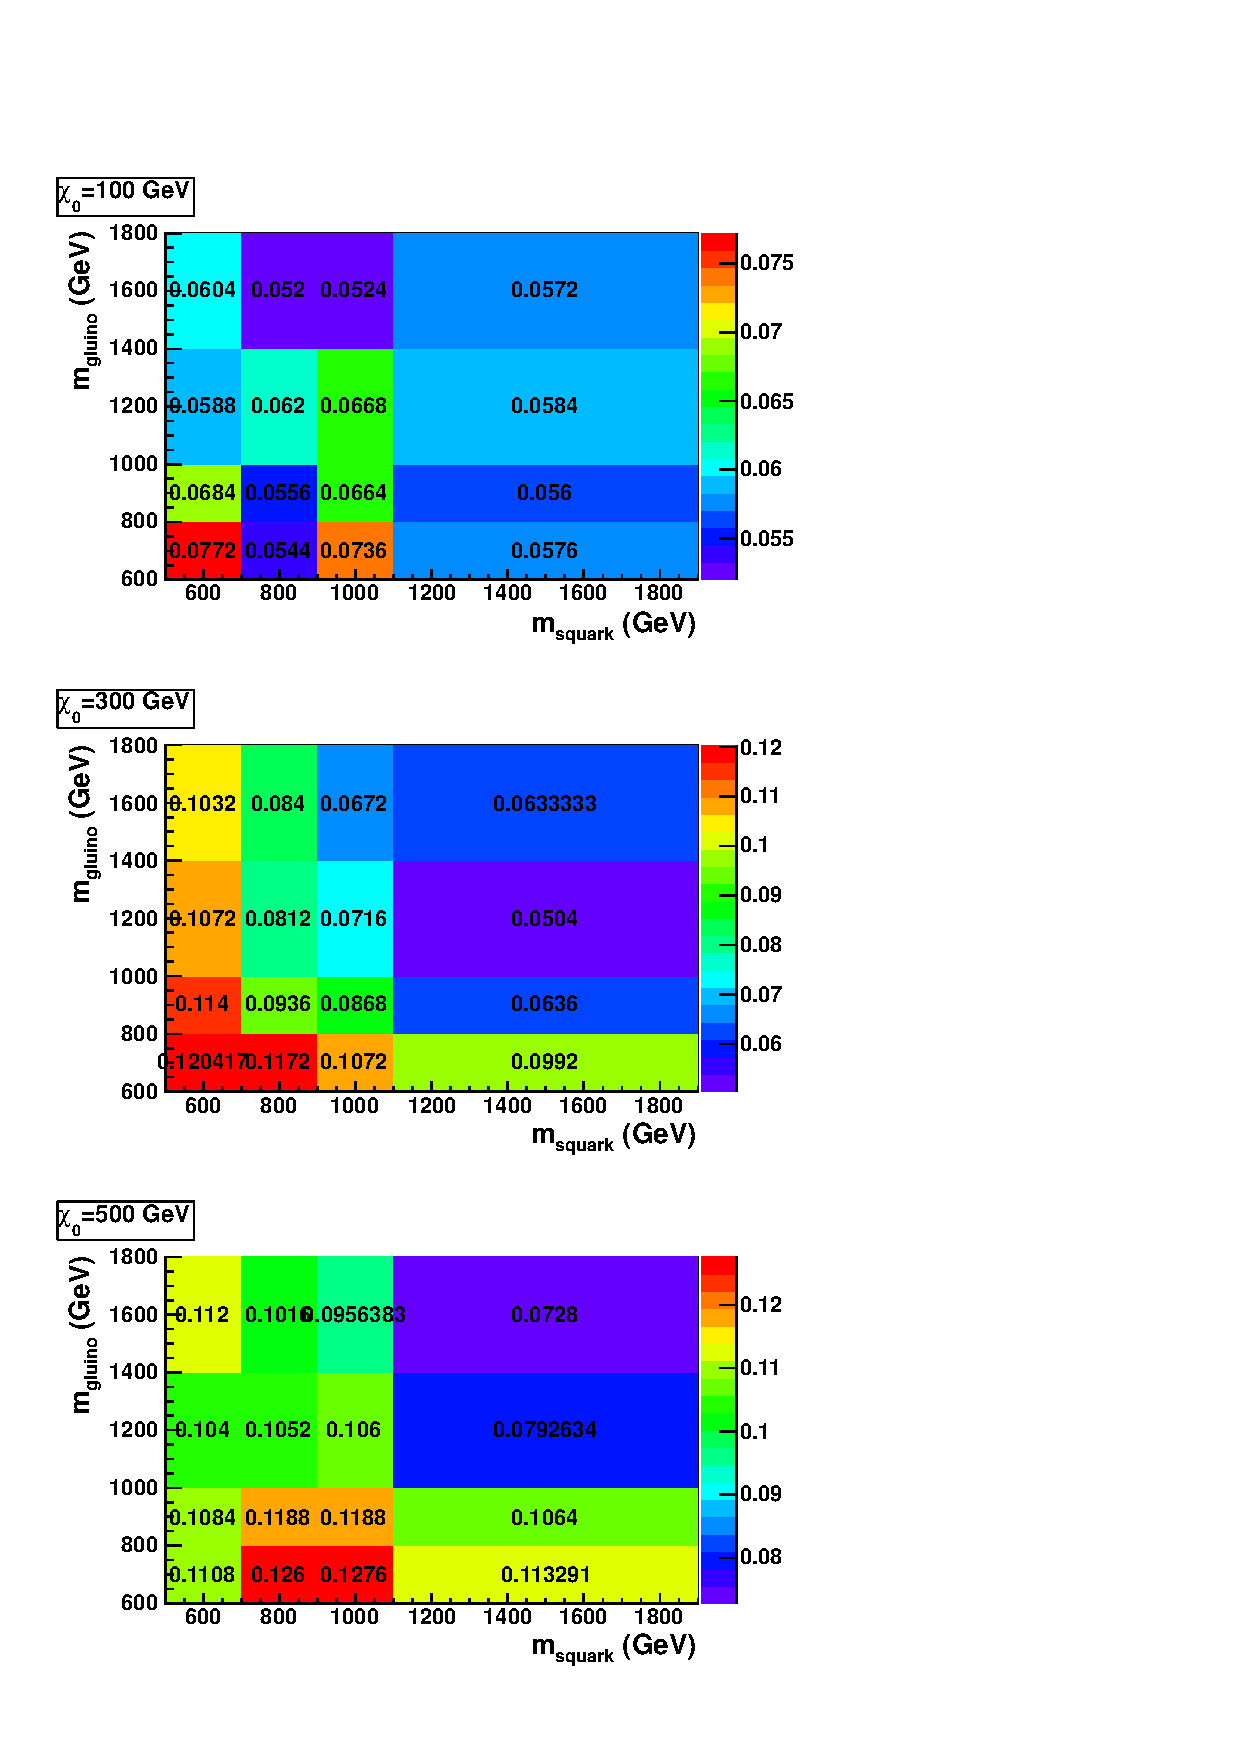
\includegraphics[width=0.45\textwidth]{figures/trigPhoton3226.pdf}
 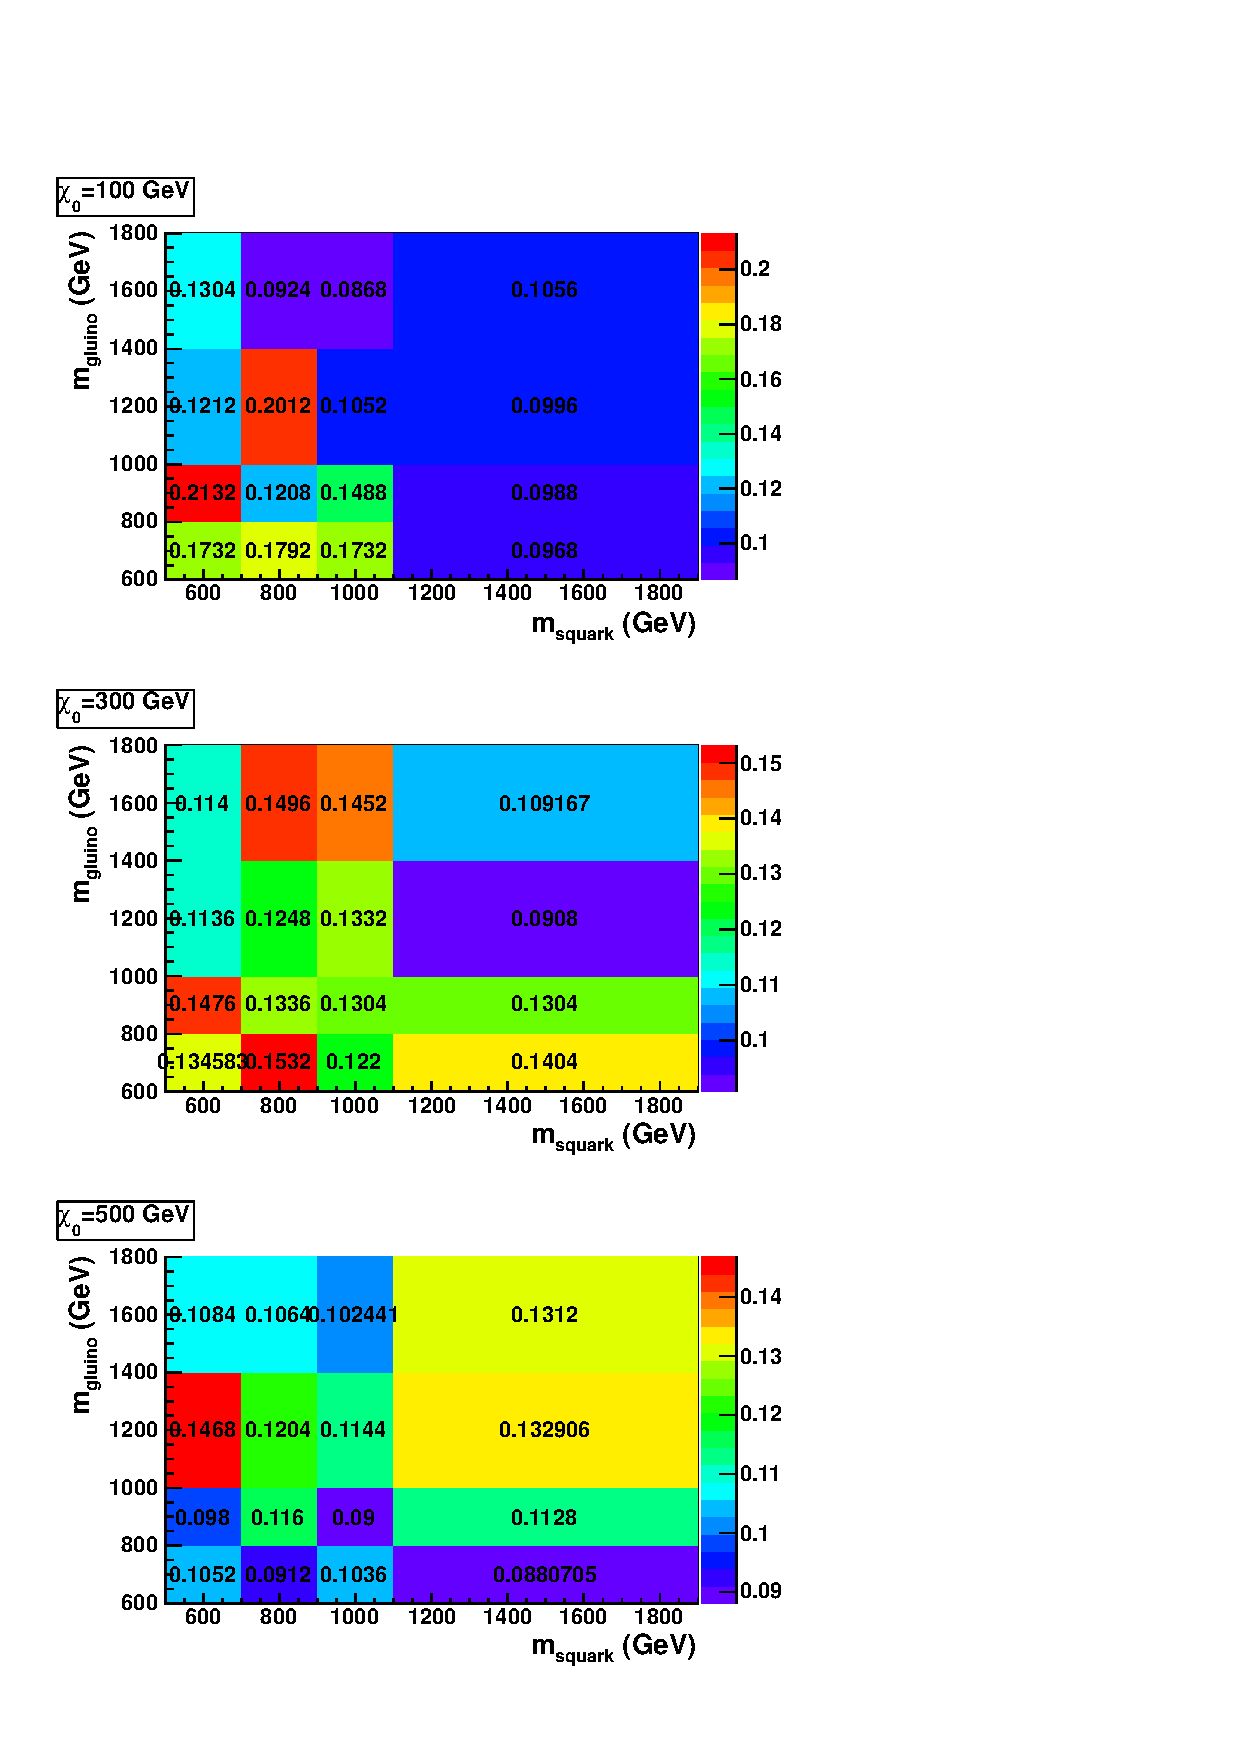
\includegraphics[width=0.45\textwidth]{figures/Photon3226.pdf}

\caption{Percent of MC in each of the 48 bins which pass the HLT\_Photon32\_Photon26\_CaloIdL\_v1 trigger 
(left) and an offline selection of a 32 GeV and 26 GeV photon with calorimeter isolation imposed}
\label{fig:diphotrigs}
\end{figure}

 \begin{figure}[!ht]
  \centering
 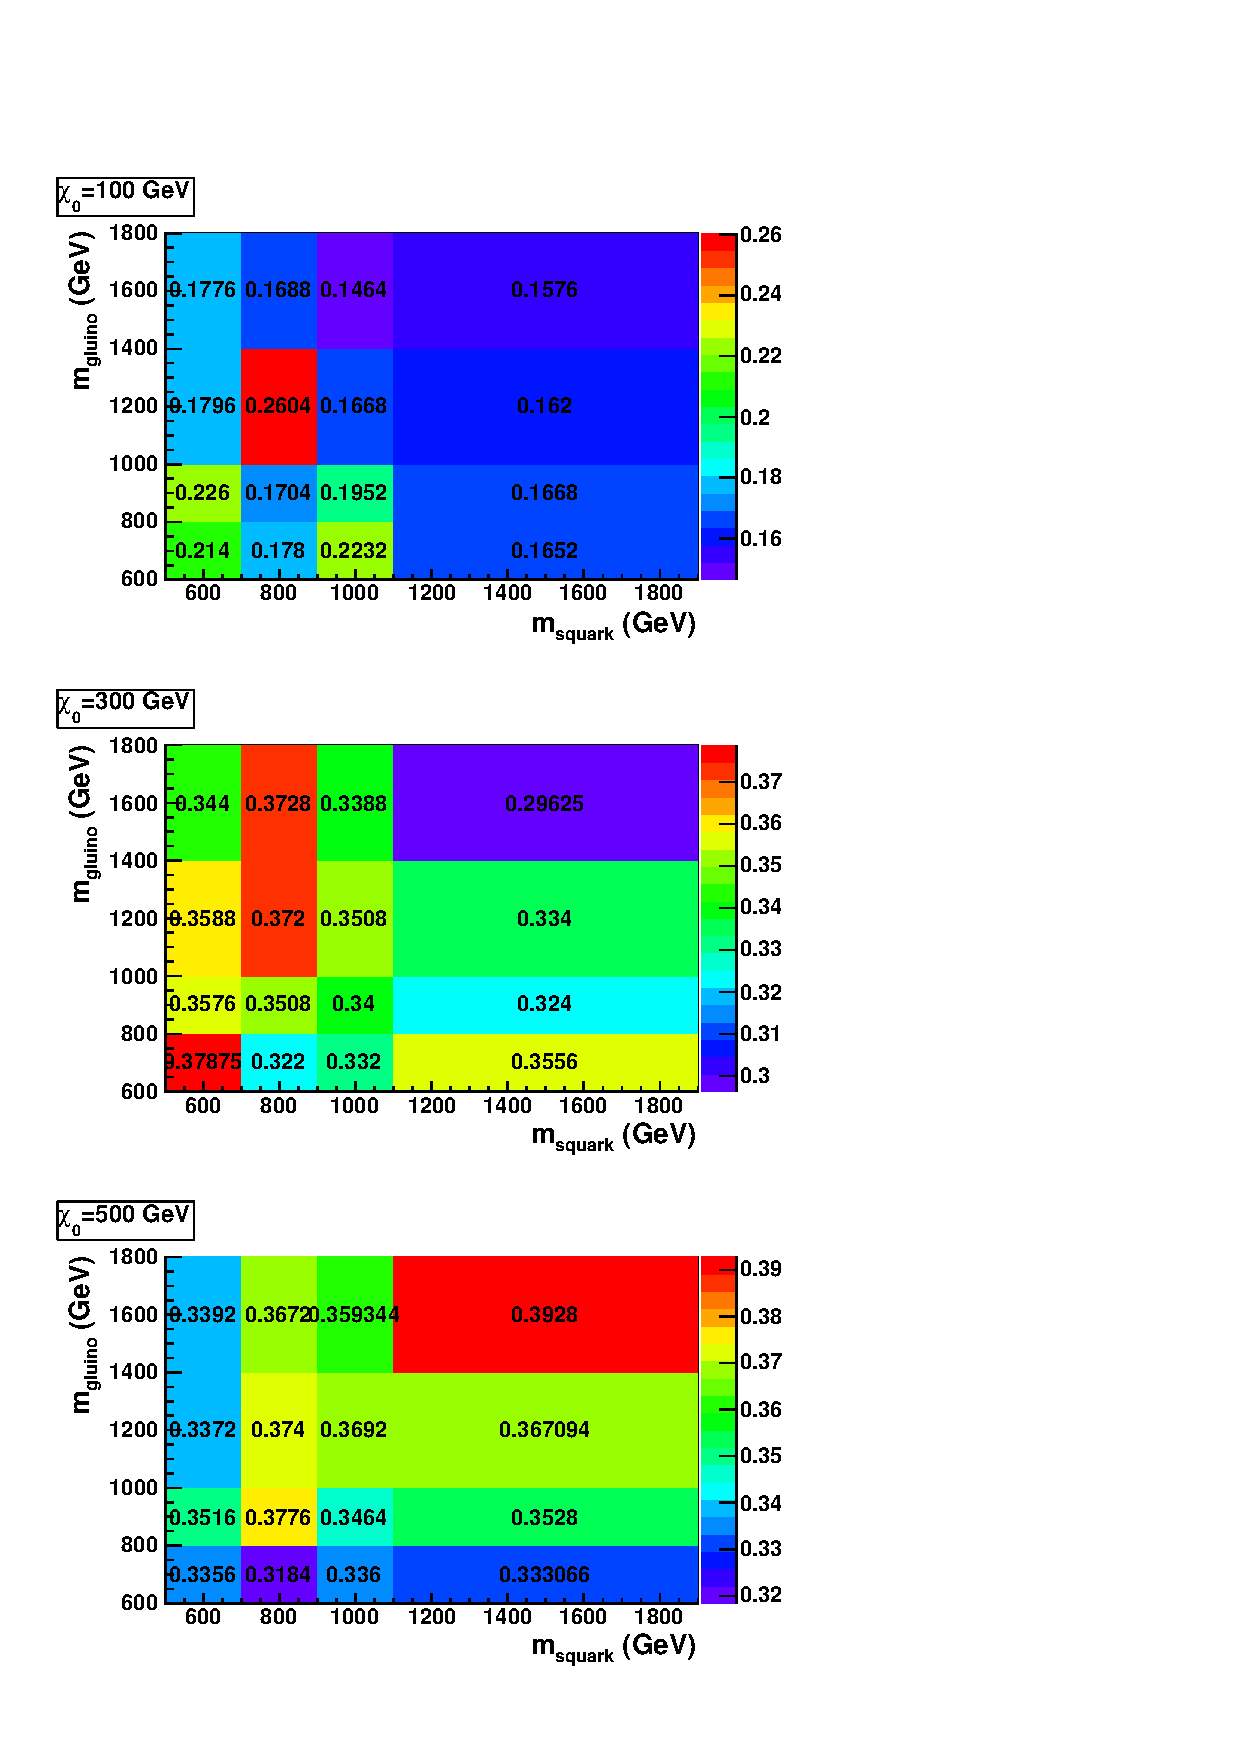
\includegraphics[width=0.45\textwidth]{figures/Photon70MHT30noPU.pdf}
 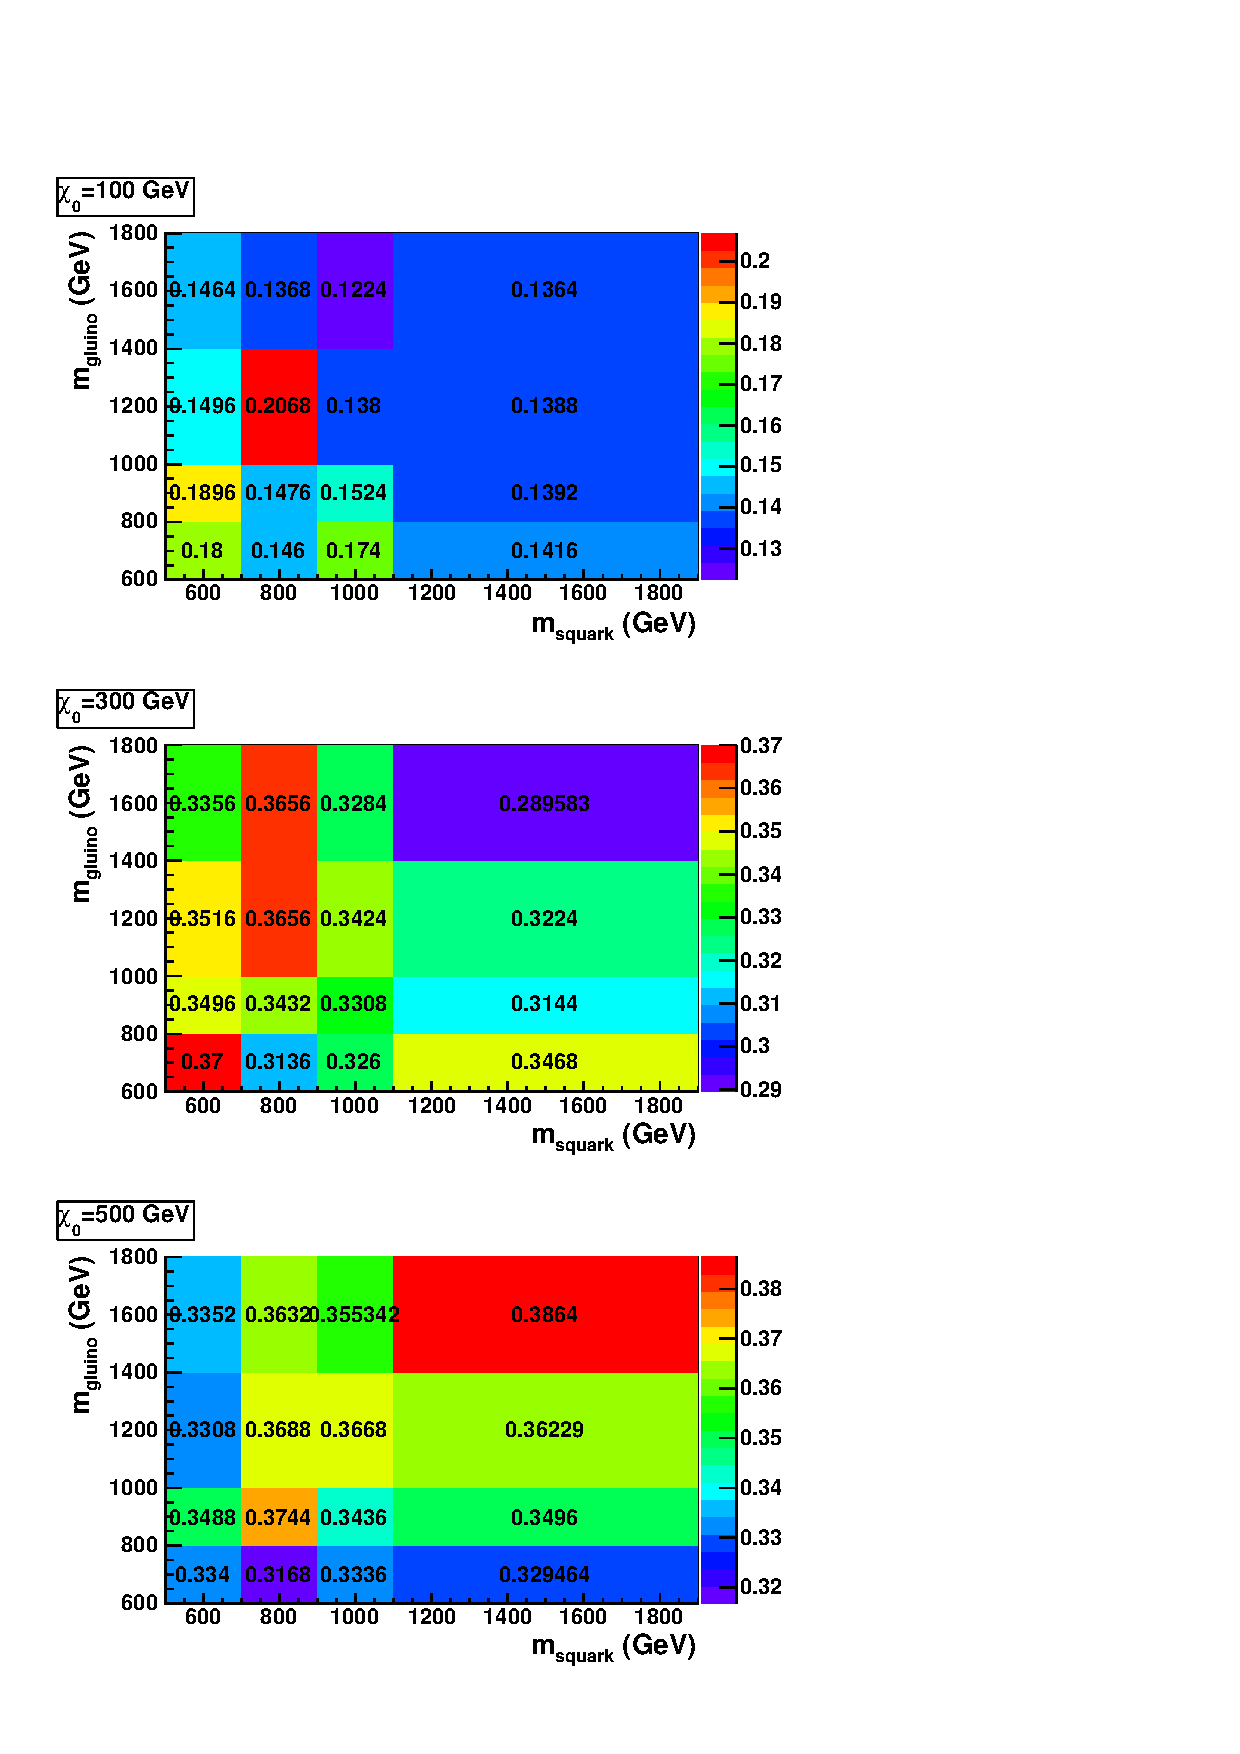
\includegraphics[width=0.45\textwidth]{figures/Photon70MHT50noPU.pdf}

\caption{Percent of MC in each of the 48 bins which pass offline requirements of a 70 GeV photon
and MHT of 30 GeV (left) and 50 GeV (right)}
\label{fig:phomhttrigs}
\end{figure}

 \begin{figure}[!ht]
  \centering
 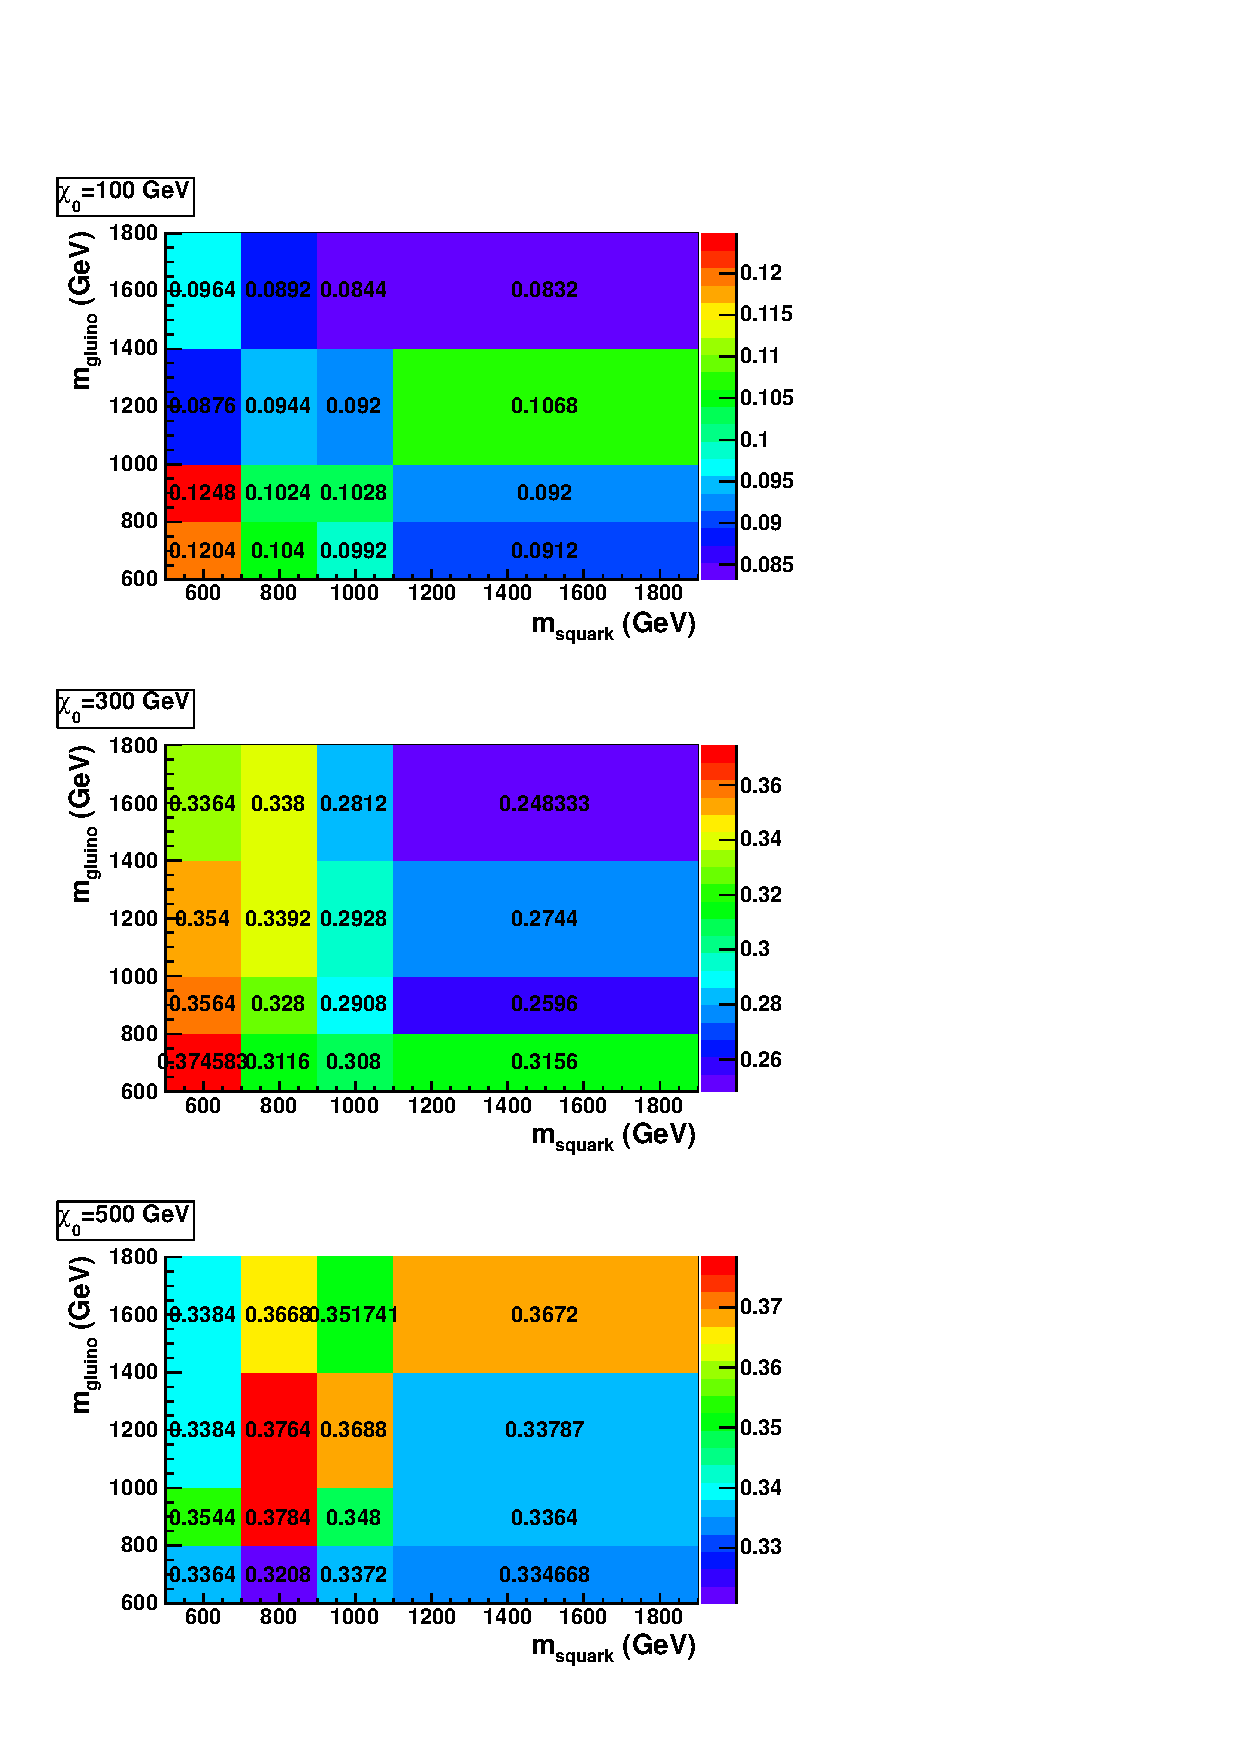
\includegraphics[width=0.45\textwidth]{figures/Photon70HT200noPU.pdf}
 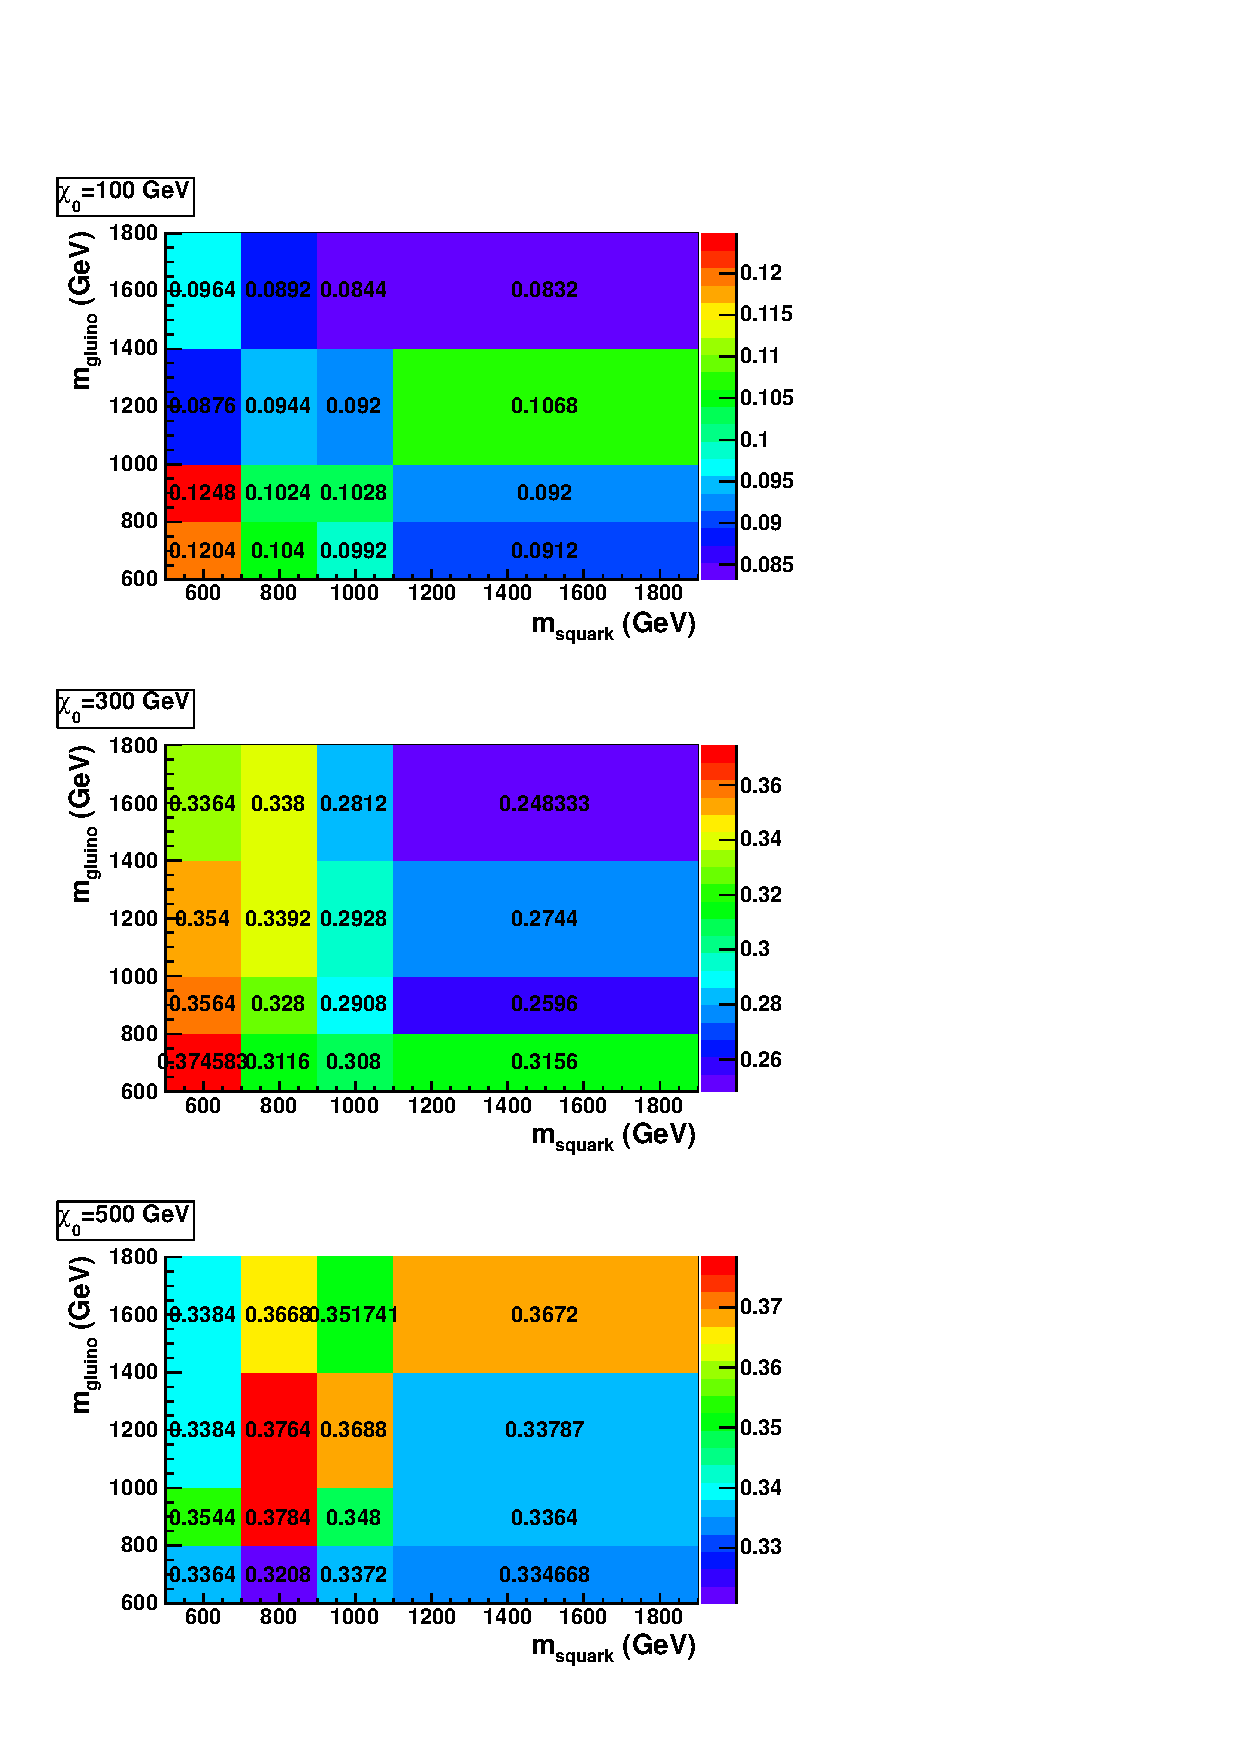
\includegraphics[width=0.45\textwidth]{figures/Photon70HT300noPU.pdf}

\caption{Percent of MC in each of the 48 bins which pass offline requirements of a 70 GeV photon
and HT of 200 GeV (left) and 300 GeV (right)}
\label{fig:phohttrigs}
\end{figure}


\subsubsection{Other useful triggers}


